\chapter{Basics}
\label{chapter:basics}
    
    In order to reach the defined goals of this thesis, more profound knowledge in different areas is necessary.
    Besides Cloud Computing and virtualization, common characteristics and features of embedded systems should be known as well.
    Also, familiarization and understanding of OpenStack are crucial.    
    This chapter aims at establishing the fundamentals needed to understand this thesis.
    
    
    %----------------------------------------------------------------------------------------
    %	Cloud Computing
    %----------------------------------------------------------------------------------------
    \section{Cloud Computing}
    \label{section:cloud}
        
        Considering the importance and extensive usage of Cloud Computing in today's world, it is hard to define the exact meaning.
        In 2011, the \ac{NIST} defined \textsl{Cloud Computing} in a special publication. 
        According to \ac{NIST}, Cloud Computing enables \textsl{"ubiquitous, convenient, on-demand network access to a shared pool of configurable computing resources (e.g., networks, servers, storage, applications, and services) that can be rapidly provisioned and released with minimal management effort or service provider interaction"} \cite{Mell2011}.
        Due to the broad utilization of Cloud Computing through third parties like Amazon or Microsoft, terms like pay-as-you-go or payment, in general, are often perceived as part of the definition \cite{Repschlager2010,Amazon2020}.
        Although this often applies, strictly reviewing, Cloud Computing only refers to the provisioning of resources.
        The business models of companies do not relate to the concept itself.
        
        \noindent Additionally, in \cite{Mell2011} \ac{NIST} established five essential characteristics of Cloud Computing.
        Through \textsl{on-demand self-service} and \textsl{broad network access}, consumers can provision computing capabilities without human interaction over the network.
        The providers' \text{resource pooling} allows serving computing resources to multiple consumers.
        \textsl{Rapid elasticity} and a \textsl{measured service} automatically control and optimize resource use by elastically provisioning and releasing them.
        
        \subsection{Service Models}
        \label{subsection:models}
        
            As mentioned previously, the main component of Cloud Computing is the provisioning of resources.
            This provisioning can be done on different levels, enabling different possibilities for the user.
            \ac{NIST} defined the following three service models for Cloud Computing, depicted by Figure \ref{figure:cloud_service_models}.
            
            \noindent \textbf{\ac{SaaS}} 
            As the name suggests, only the software is provisioned.
            In this model, the software is executed on cloud infrastructure and consumers can access it through thin-client interfaces like web browsers.
            The consumers do not manage or even have access to the underlying cloud infrastructure or the environment like the \ac{OS}.
            
            \noindent \textbf{\ac{PaaS}} 
            The service provisioned here is a platform for deployment of applications.
            The provider offers control over deployed applications and possibly over environmental settings for hosting applications.
            The consumers do not manage or even have access to the underlying cloud infrastructure.
            
            \noindent \textbf{\ac{IaaS}} 
            The consumer has access to fundamental computing resources and is able to provision them.
            The user has no access or control over the underlying hardware but can run arbitrary software and control the \ac{OS}, storage, and deployed applications.
            This thesis aims at establishing an \ac{IaaS} cloud on the automotive hardware presented in Chapter \ref{chapter:host_and_Test_setup} using OpenStack.
            
            \begin{figure}[ht]
                \begin{center} 
                    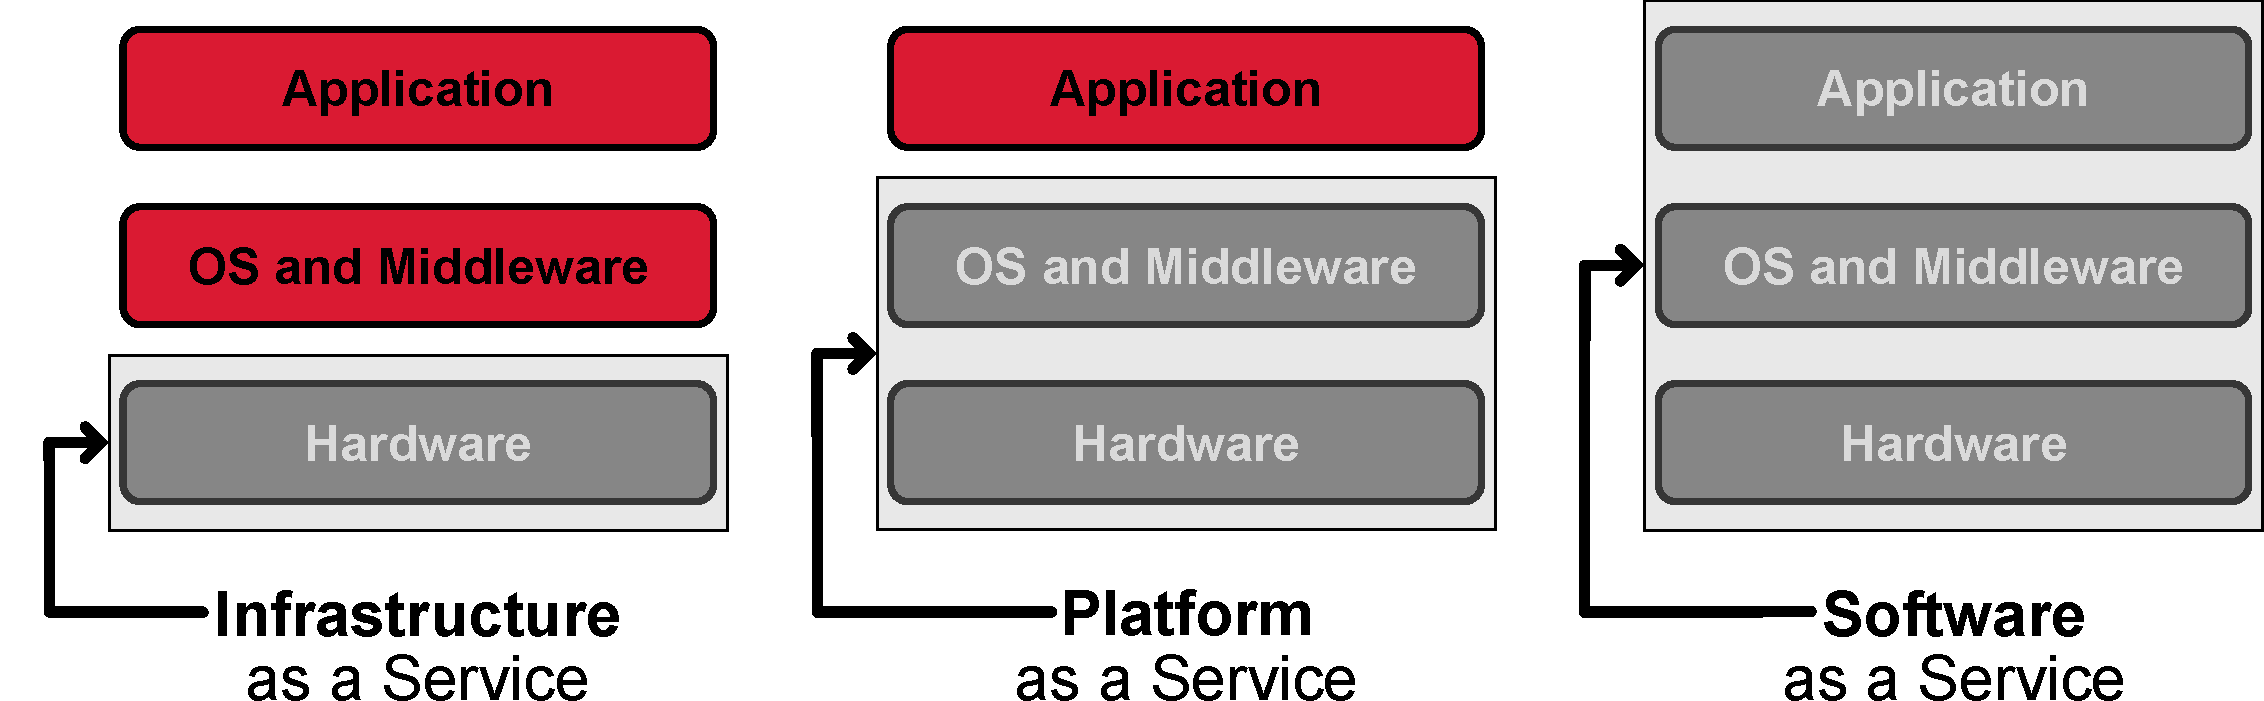
\includegraphics[width=\textwidth ]{02_service_models.pdf} 
                    \caption{Cloud computing service models}
                    \label{figure:cloud_service_models}
                \end{center}	
            \end{figure}
        
        
        \subsection{Architectures}
        \label{subsection:architecture}
            
            Except for different service models, Cloud Computing can be characterized by its architecture.
            Depending on the accessibility to the infrastructure, the following architectures are defined.
            
            \newpage
            \noindent \textbf{Private Cloud} 
            The infrastructure is available for only one organization.
            Related consumers, e.g., business units, can access and use the infrastructure.
            The infrastructure itself can be managed either by the organization itself, a third party, or a combination of both.
            Throughout this thesis, a private architecture is used, as no access for other parties is considered.
            
            \noindent \textbf{Community Cloud}
            In addition to private clouds, in community clouds, the usage is not exclusive to one organization.
            Organizations with shared interests and concerns have access to the infrastructure and can access the provided services.
            The infrastructure itself can be managed by either one of the organizations itself, a third party, or a combination of both.
            
            \noindent \textbf{Public Cloud}
            As the name suggests the cloud infrastructure is accessible by the general public for use.
            Various institutions, like businesses, academics, or governments, can be responsible for managing the cloud infrastructure.
            
            \noindent \textbf{Hybrid Cloud} 
            This infrastructure is a composition of two or more different cloud infrastructures.
            Both clouds remain unique entities but are connected to each other for, for example, data exchange.
            
        \subsection{Advantages and Disadvantages}
        \label{subsection:advantages_disadvantages}
            
            Cloud Computing is not without reason a prevalent and beneficial model.
            Various reasons exist why Cloud Computing should be adopted, from a technical and business point of view.
            However, Cloud Computing also comes with negative aspects, especially for embedded systems.
            Based on \cite{Alzahrani2014,Hallmans2015}, some advantages and disadvantages of Cloud Computing shall be pointed out.
            
            
            \subsubsection{Advantages}
            
                \noindent Cloud Computing introduces a new degree of \textbf{flexibility}. 
                Virtualizing available, distributed resources as one coherent pool makes the allocation of applications to specific systems like a specific \ac{ECU} redundant.
                
                \noindent Moreover, \textbf{scalability} and, therefore, \textbf{performance} can be tremendously improved.
                Regarding the topic of upgradability, in current embedded systems, this is not even considered or possible. 
                Through Cloud Computing, upgrading or simply adding resources, for example, computing power or memory, would instantaneously become possible. 
                Especially in today's environmentally and resource-conscious society, this could be an interesting topic.
                
                \newpage
                \noindent Additionally, Cloud Computing is ideal if \textbf{redundancy} is needed.
                Considering embedded systems with high safety requirements, this is essential.
                While today additional hardware is used, Cloud Computing could enable applications to be easily shifted or duplicated in case of hardware failure.
                Chapter \ref{chapter:usecases} examines the advantages of flexibility and redundancy in greater detail.
            
             
            \subsubsection{Disadvantages}
            
                \noindent Deploying and managing cloud infrastructures introduces a significant level of \textbf{complexity}.
                Understanding the exact behavior of the whole software or software components becomes impossible.
                
                \noindent This introduces new problems in the areas of \textbf{security}.
                Especially for embedded systems, where updating software is not necessarily intended, security flaws and vulnerabilities are critical.
                With big and complex software, vulnerabilities can be overlooked and later discovered during production.
                While in data centers, this can quickly be resolved through updates, embedded systems are scarcely updated.
                Using cloud infrastructure could therefore create a conflict with this tradition
                
                \noindent Further, this contradicts embedded systems with high safety requirements that must have \textbf{deterministic behavior}.
                Besides the inability to understand the whole software, possible exploitation of security flaws adds to the fact that it is impossible to know the software's behavior with confidence. 
            
    
    %----------------------------------------------------------------------------------------
    %	Virtualization
    %----------------------------------------------------------------------------------------
    \section{Virtualization}
    \label{section:virtualization}
    
        Cloud Computing relies on the provisioning of resources. 
        To do that, resources like the \ac{CPU}, \ac{CPU} cycles, or memory have to be virtualized.
        Virtualization describes a real-world object's mapping onto a virtual object with the same or similar properties \cite{Garbacki2007}.
        This allows applications and services to be deployed onto the virtualized hardware instead of directly onto the physical resources.
        From now on, the hardware providing the resources is called the \textsl{host}, while the software, for example, a \ac{VM}, using those resources is called the \textsl{guest}.
        The management of the virtualized resources is handled by a software called \textsl{hypervisor}.
        The following subsections will describe two common concepts of virtualization, as well as two common hypervisors using these concepts.
        
        
        \subsection{Hypervisors}
        \label{subsection:hypervisors}
        
            Hypervisors are systems or pieces of software initially developed for monitoring purposes in virtual computing \cite{Blenk2016}.
            In addition, hypervisors are responsible for the allocation of physical resources to individual guests.
            Guest \acp{VM}, for example, can execute their own \ac{OS} and run as an individual computing platform.
            By providing a hardware abstraction layer, hypervisors provide interfaces for guests to interact with the physical hardware.
            Two widely used hypervisors are \ac{KVM} and XEN.
            In this thesis, the OpenStack cluster will use \ac{KVM} as the hypervisor.
        
        
        \subsection{Virtualization Concepts}
        \label{subsection:concepts}
        
            For the virtualization of resources, especially the \ac{CPU} and \ac{CPU} cycles, two main approaches established themselves.
            Their main difference resides in the hypervisor and the hypervisors reaction to non-virtualizable machine instructions.
            During execution, atomic machine instructions define the actions performed by the processor. 
            While most machine instructions are independent of specific architectures, some instructions behave differently or require specific privileges \cite{Marinescu2018}.
            As stated by Popeck and Goldberg already in 1974, to provide efficient behavior to guests, a certain percentage of instructions must be executed without the hypervisors intervention \cite{Popek1974}.
            In cases where hypervisors' interventions are necessary, the instructions require a specific behavior not known by the hardware. 
            To resolve such non-virtualizable instructions, two different strategies can be used, resulting in two different virtualization approaches visualized by Figure \ref{figure:full_para_virtualization}.
            
            \noindent \textbf{Full-Virtualization} 
            Guests run on a hardware abstraction layer, being an exact copy of the host hardware \cite{Marinescu2018}. 
            In the case of non-virtualizable instructions, the hypervisor identifies these instructions in memory during execution and replaces them with suitable instructions \cite{Binu2011}.
            The guest is not aware of this replacement and continues its execution unhindered.
            Therefore, no modifications need to be performed to the guest system in advance, but the host hardware must support hardware virtualization to provide an efficient solution. 
            \ac{KVM} is a widely adopted hypervisor using full-virtualization.
            
            \noindent \textbf{Para-Virtualization} 
            Guests run on a hardware abstraction layer, being a slightly modified copy of the host hardware \cite{Marinescu2018}. 
            In the case of non-virtualizable instructions, the hypervisor provides a specific interface to the virtualized hardware to translate these instructions \cite{Binu2011}.
            The guest must be extended with specific drivers to make use of this interface.
            Therefore modifications to the guest are needed, but contrary to full-virtualization, para-virtualization does not require hardware support for virtualization.
            XEN is a popular hypervisor using para-virtualization.
            
            \begin{figure}[ht]
                \begin{center} 
                    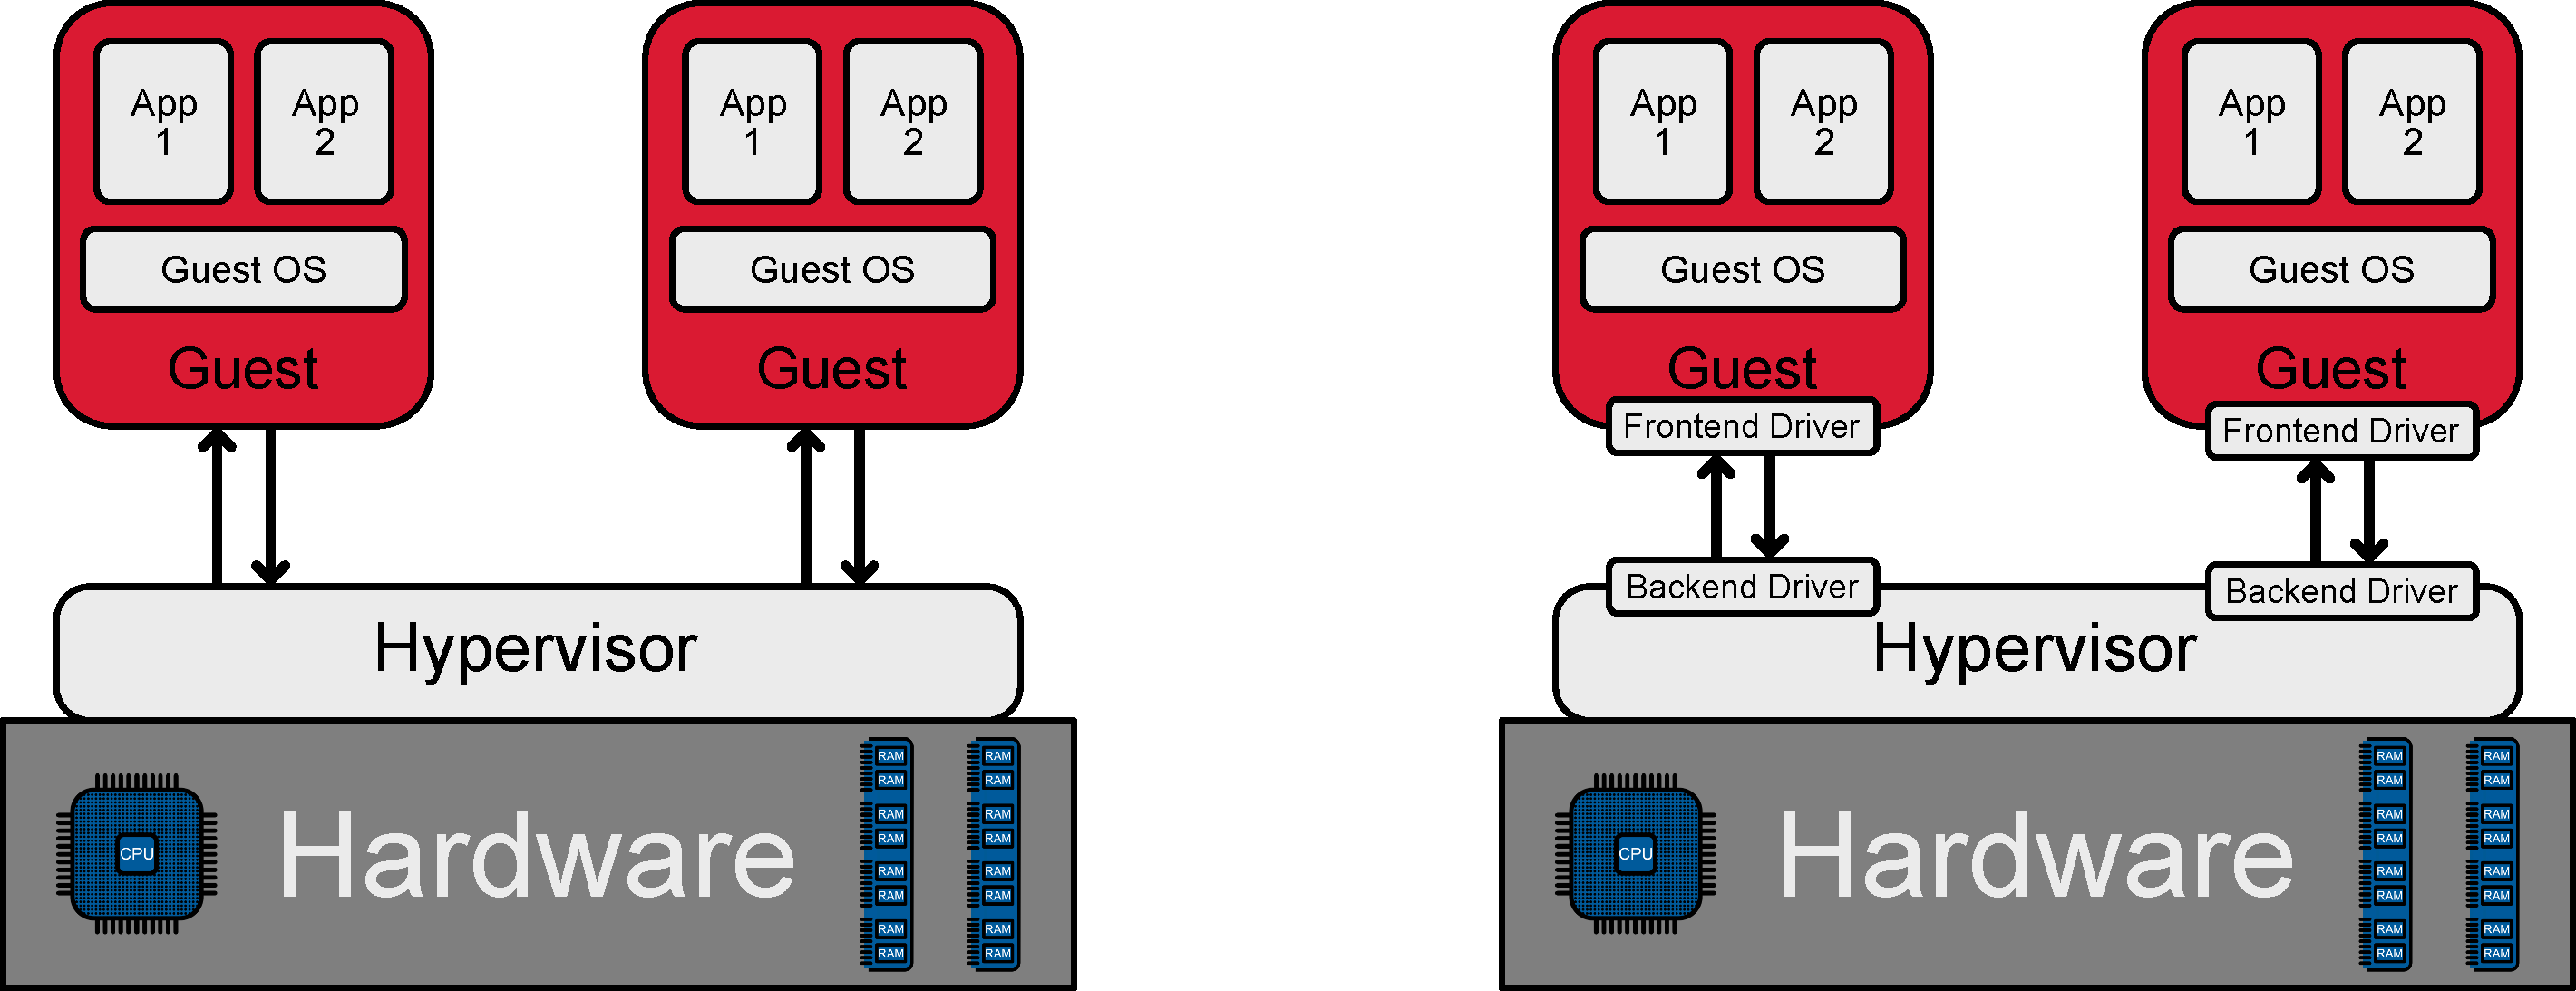
\includegraphics[width=\textwidth]{02_virt_concepts} 
                    \caption[Full-Virtualization and Para-Virtualization]{Full-Virtualization (left)  and Para-Virtualization (right)}
                    \label{figure:full_para_virtualization}
                \end{center}	
             \end{figure}

        
    %----------------------------------------------------------------------------------------
    %	Embedded Systems
    %----------------------------------------------------------------------------------------
    \section{Embedded Systems}
    \label{section:embedded}
    
        In today's world, embedded systems are widely adopted and in use.
        From areas like robotics and the Internet of Things, over automotive and avionic systems to nuclear power plants, embedded systems perform various essential tasks.
        Although these areas all come with different requirements, the function of embedded systems mostly stays the same.
        P. Marwedel defined embedded systems as \textsl{"information processing systems embedded into enclosing products"} \cite{Marwedel2018}.
        Often, embedded systems are linked to the physical world and interact with physical processes.
        In such cases, the systems can be named \textsl{Cyber-Physical Systems}. 
        In \cite{Lee2007}, E. Lee defined Cyber-Physical Systems as \textsl{"integrations of computation and physical processes"}.
        The following sections are based on P. Marwedel's book on Embedded Systems Foundations of Cyber-Physical Systems \cite{Marwedel2018}.
        
        
        \subsection{Characteristics}
        \label{subsection:characteristics}
        
            Despite different environments, embedded systems share several characteristics and challenges these systems have to meet.
            According to P. Marwedel, the following attributes are commonly found:
            
           \noindent \textbf{Dependability} 
            Due to the direct interaction with the environment, embedded systems have an immediate effect and impact on the physical world.
            Additionally, as described later, the lack of a minimal user interface makes a human reaction in case of failure or misbehavior very hard or even impossible.
            Therefore, embedded systems must be dependable by providing safety, security, confidentiality, reliability, maintainability, and availability.
            
           \noindent \textbf{Time Constraints}
            The interaction with physical processes binds the execution or computation of specific things to determined deadlines.
            Depending on the computation and the physical process involved, these limits can be either short or long.
            Moreover, depending on the physical process, a deadline miss can be either catastrophic or less noticeable. 
            
           \noindent \textbf{Resource Awareness}
            Representing not the primary system but being embedded into an encapsulating product, embedded systems often are restricted in various resources.
            Resources like code size and performance or run-time efficiency are optimized as far as possible. 
            Through this, further resources like energy, weight, or space can be optimized.
            Due to very high production volumes of embedded systems, for example, automotive \acp{ECU}, the cost is a crucial factor.
            By minimizing any resource usage, general costs can be reduced, which is very much desirable.            

           \noindent \textbf{Dedicated User Interface}
            The integration into encapsulating products implies that the interaction will most probably happen with the outer product.
            Therefore, user interfaces of embedded systems are specific to the application and held as minimal as possible.
            If no interaction is anticipated, no user interface is provided. 
            Only interfaces for debugging or flashing may then be implemented, consisting of simple switches or interfaces for console access.
        
              
        \subsection{Software}
        \label{subsection:software}
        
            To successfully overcome challenges like time constrains and dependability, \acp{OS} for embedded systems are specially tailored.
            Limited resources and defined applications make it possible and necessary to specifically configure \acp{OS} according to individual needs.
            The lack of untested and unnecessary software allows the assumption about the presence of only reliable and safe software, which further allows to leave out standard protection mechanisms.
            For the embedded environment, access to \ac{OS} service calls or interrupts is essential to react fast and on time to specific events, like sensor data.
            As many embedded systems do not underlie only time constraints but must be real-time capable, further functionality is required by the \ac{OS}.
            
            \noindent \textbf{Real-Time OS}
            Real-Time \acp{OS} are necessary for the construction of real-time systems.
            Real-Time systems describe systems, which not only depend on the functional correctness but equally depend on the in-time computation of results.
            In other words, a particular deadline for a computation must not be missed, or else catastrophic events could occur.
            To ensure such deadlines are not missed, real-time \acp{OS} must provide very predictable timing.
            The OS must manage the scheduling of threads, processes, and tasks through appropriate scheduling algorithms to enable an in-time computation of every task.            
            Naturally, the \ac{OS} must additionally be fast and deliver a good performance.
            These requirements are achieved through the use of fast, customized, and proprietary kernels, as well as with real-time extensions to standard \acp{OS}.
            
            \noindent \textbf{Embedded Linux}
            With more complex applications and more requirements, embedded \acp{OS} must provide increased functionality.
            When developing new software components and integrating them, using an existing and extensively tested \ac{OS} can be preferable.
            Using Linux, which relies on an Open-Source kernel, eliminates commercial costs and allows the kernel's desired configurability.
            The primary target environment for Linux being servers and desktops, Linux is designed for general-purpose computing.
            Aiming for high average performance and fair scheduling, additional scheduling policies must be added to the kernel to satisfy real-time requirements.
            Similarly, the usage of memory differs in desktop and server environments.
            While in desktop and server environments, the memory is often used for caching, this is a waste of resources in the context of embedded systems.
            Although there are techniques to eliminate this duplication of memory, they come at the cost of high complexity and often more expensive storage solutions.
            This again leads to the reconsideration of allowing, for example, swap space and using larger memory.             
   
   
    %----------------------------------------------------------------------------------------
    %	 OpenStack
    %----------------------------------------------------------------------------------------
    \section{OpenStack}
    \label{section:openstack}
        
        OpenStack is a free and Open-Source Cloud Computing software.
        It aims at providing \textsl{"a ubiquitous Open Source Cloud Computing platform that is easy to use, simple to implement, interoperable between deployments, works well at all scales, and meets the needs of users and operators of both public and private clouds”} \cite{OpenStackH2018}.
        In other words, OpenStack enables the deployment of own clouds on the hardware of choice. 
        The project itself originated from two separate projects at Rackspace and Anso Labs, developing both the corresponding counterparts for each other.
        In 2010, the project OpenStack was officially announced and the first release published.
        At the time of writing, 22 releases happened, with the newest one having the series name \textsl{Victoria}.
        This release was used throughout this thesis for all OpenStack software and components.
        
        \noindent OpenStack is built upon multiple different software components, each providing specific functionality.
        Currently, OpenStack consists of 45 different components.
        Figure \ref{figure:openstack_map} shows all available OpenStack software components along with additional software and tools.
        The relevant components for this thesis will be presented in the next section.
        
        \begin{figure}[ht]
            \begin{center} 
                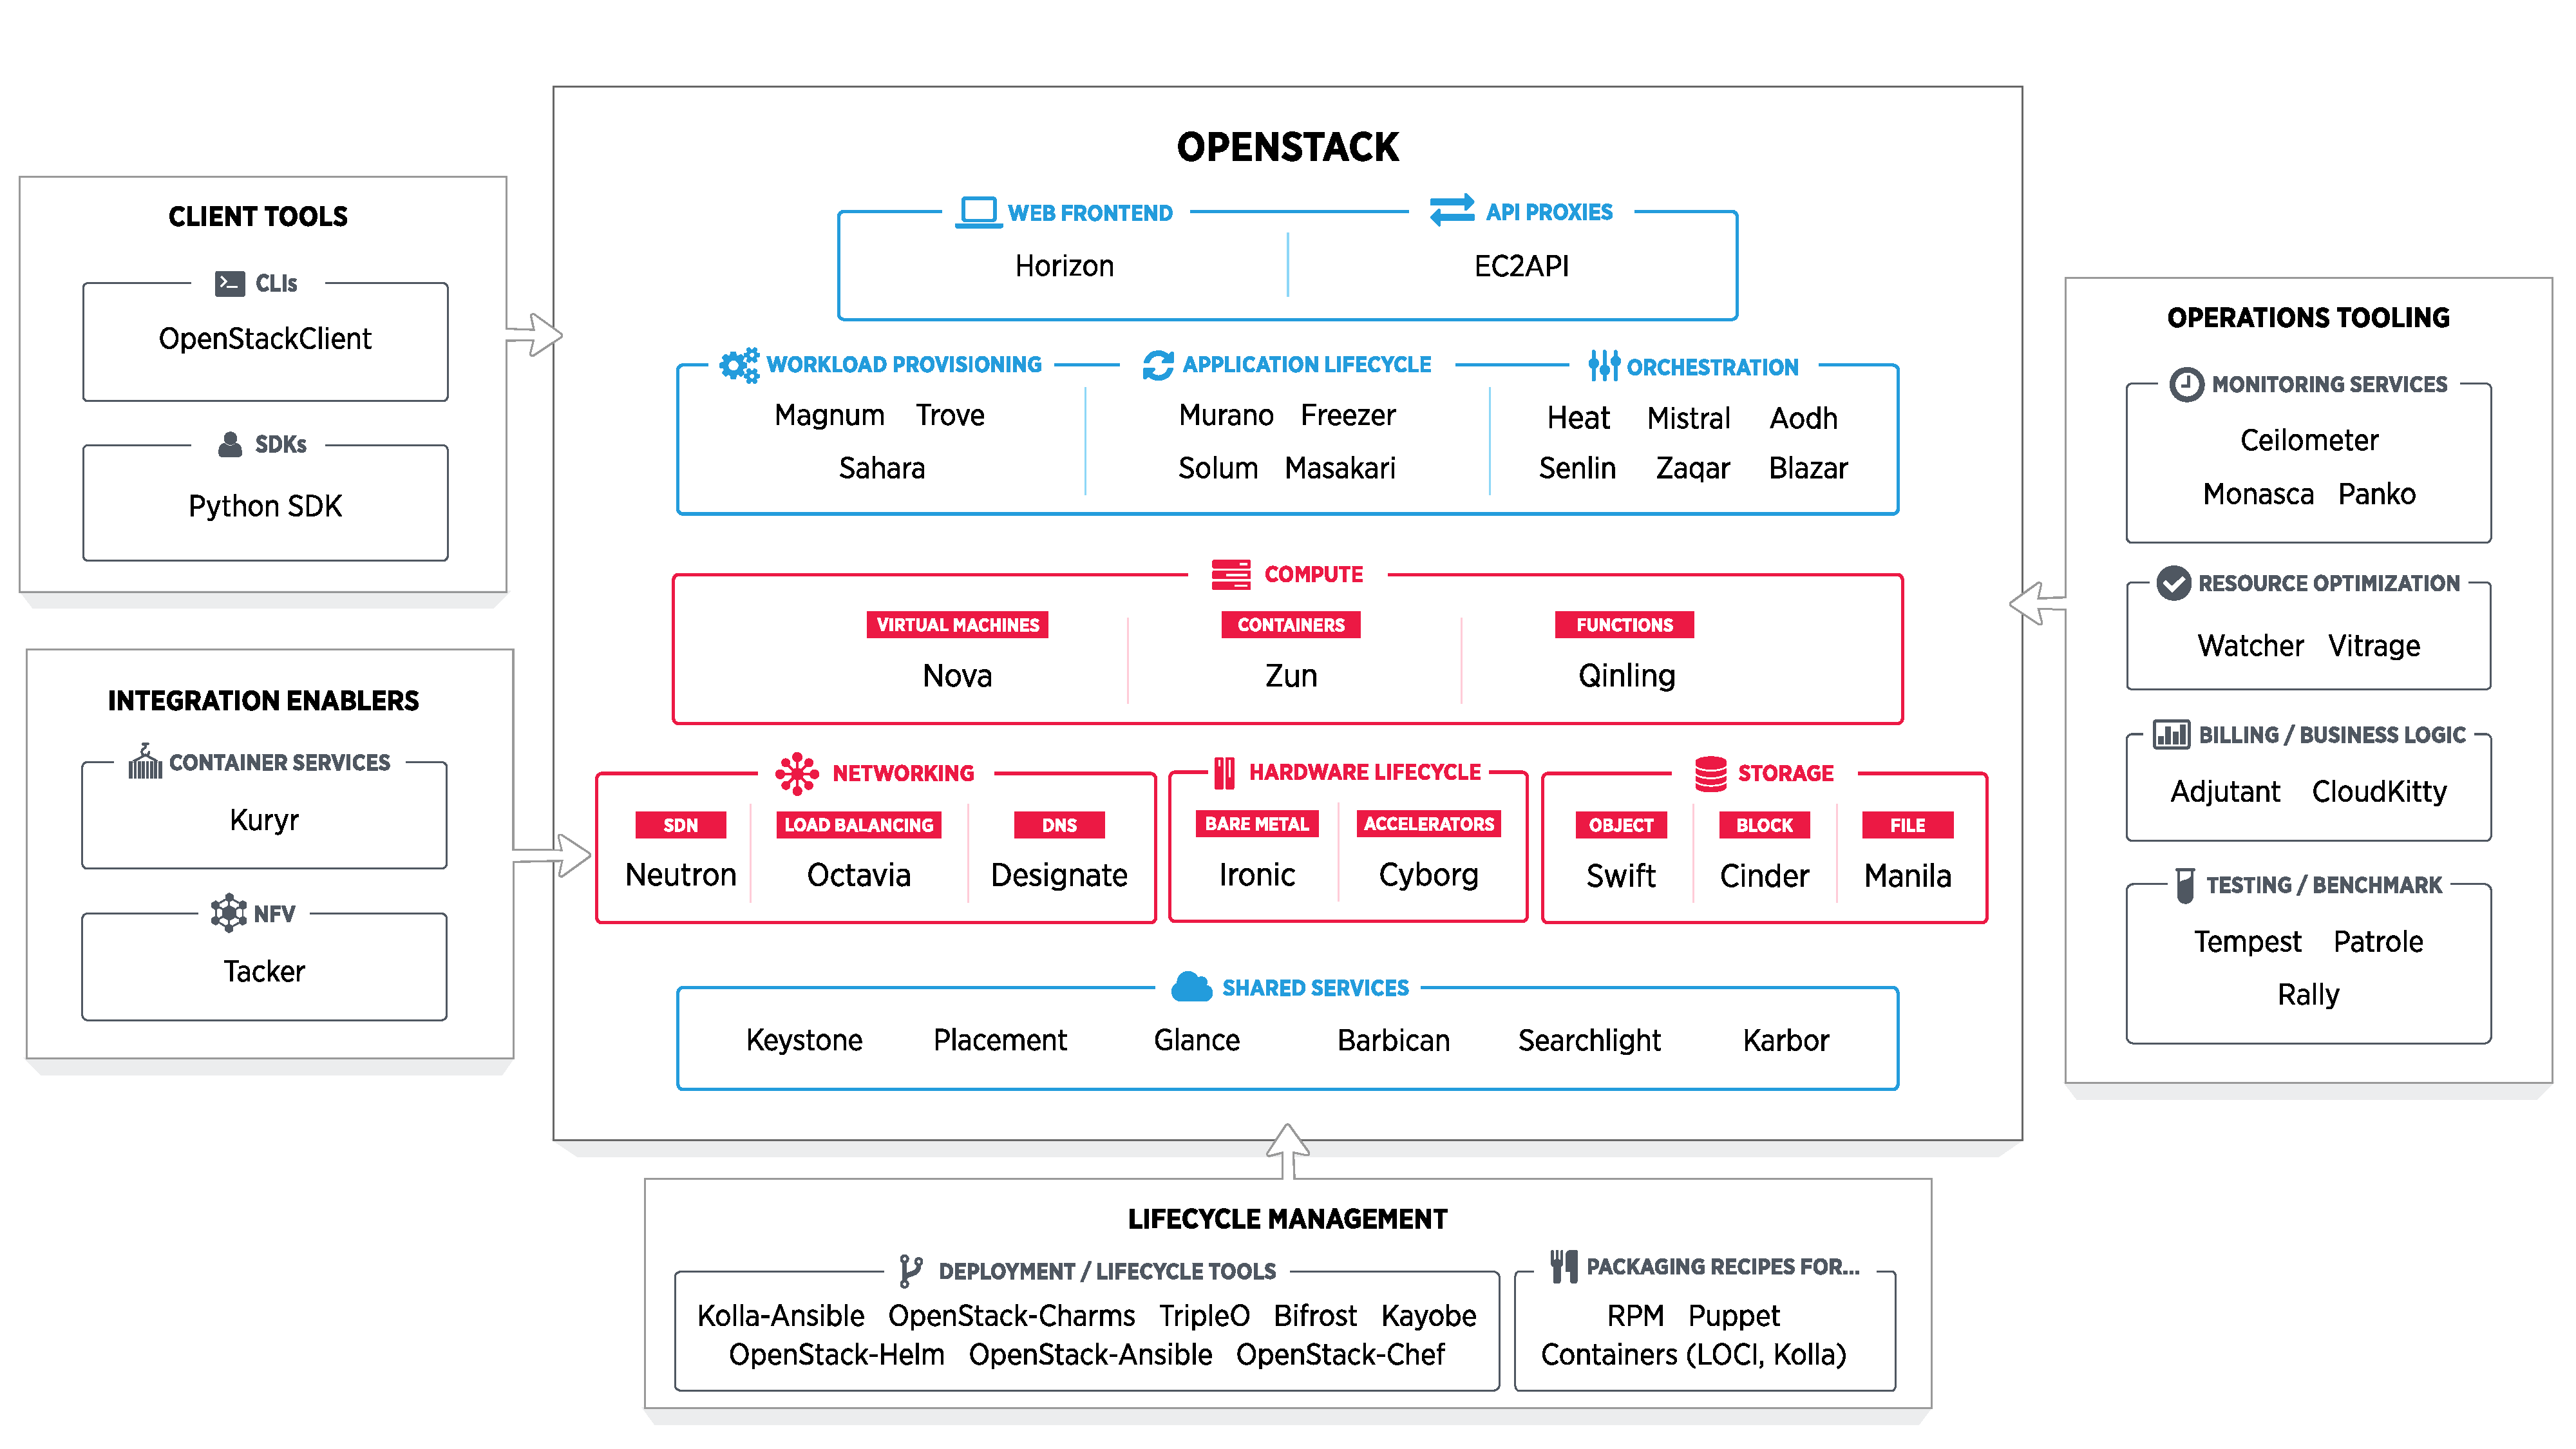
\includegraphics[width=\textwidth ]{02_openstack-map} 
                \caption[Map of OpenStack's software landscape]{Map of the OpenStack's software landscape \cite{OpenStackL2020}}
                \label{figure:openstack_map}
            \end{center}	
         \end{figure}
         
        \noindent With OpenStack's numerous components and their primarily intended environment being data centers, an OpenStack cluster is designed to consist of multiple hosts.
        However, it is possible to install and execute all services on one host.
        Commonly, an OpenStack cluster consists of one controller node and multiple compute nodes.
        Depending on the goals and resources, dedicated storage and networking nodes are possible.
        Throughout this thesis, only dedicated compute nodes will exist, while all other services and components will be executed on one controller node.


        \subsection{Software Components}
        \label{subsection:components}
            
            As depicted in Figure \ref{figure:openstack_map}, many different software components exist.
            For the scope of this thesis, only the crucial components of an OpenStack cluster will be used.
            Figure \ref{figure:openstack_components} illustrates these components along with their interactions.
            The following sections briefly describe these components.
            
            \begin{figure}[ht]
                \begin{center} 
                    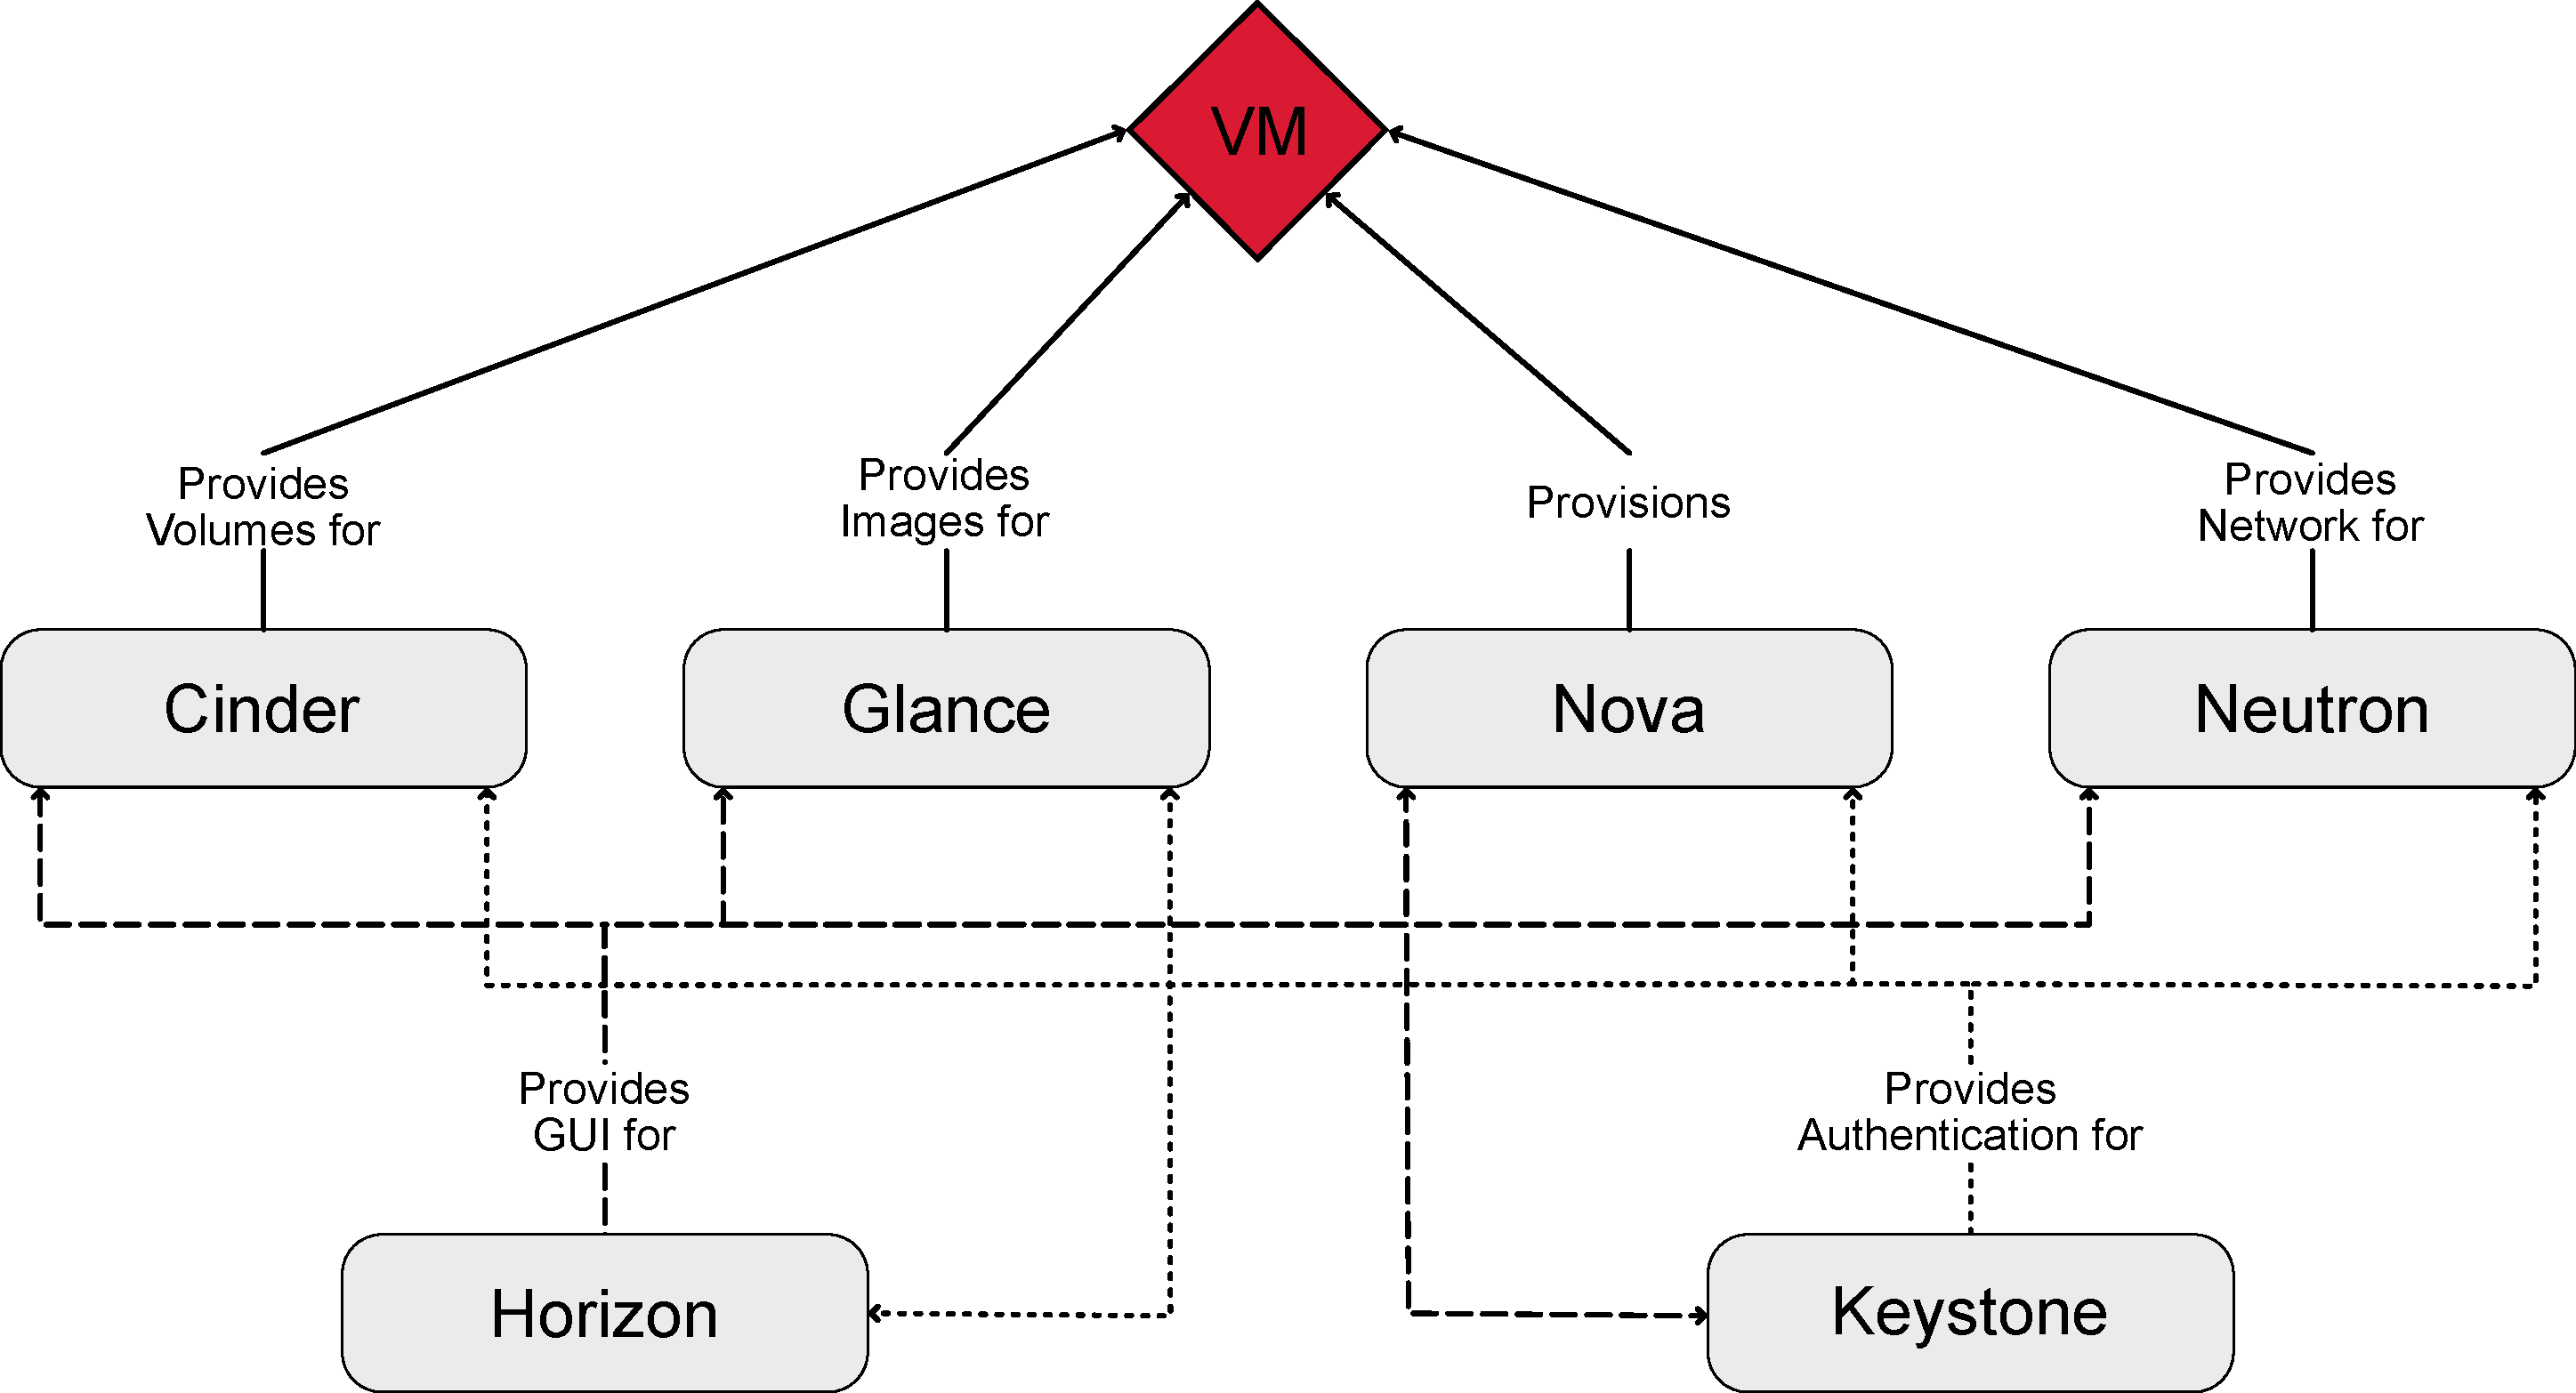
\includegraphics[width=0.7\textwidth ]{02_openstack-components.pdf} 
                    \caption[Interaction of OpenStack components]{Interaction of OpenStack components \cite{UnixArena2015}}
                    \label{figure:openstack_components}
                \end{center}	
             \end{figure}
             
             
             \subsubsection{Shared Services}
             
                Regarding shared services, the identity service \textsl{Keystone} and \textsl{Glance} are critical to a functioning OpenStack cluster.
                
                \noindent \textsl{Keystone} provides authentication for clients in the OpenStack environment. 
                Clients hereby refer to other OpenStack components, which need to authenticate their operations, as well as to actual clients, authenticating themselves to access the OpenStack cluster.
                
                \noindent \textsl{Glance} provides the functionality of registering and retrieving images for \acp{VM}.
                The actual images can be stored in various locations, and using Glance's \ac{API}, image metadata and the actual retrieval of the image is possible.
                
                \noindent Although not essential, the placement services \textsl{Placement} provides the functionality of tracking cloud resources and their usage.
                Using an API, Placement helps other services to manage and allocate their resources accordingly, which is an important factor in this thesis’s context. 
             
             
             \subsubsection{Web Frontend}
                 
                Although not strictly necessary for a functioning OpenStack Cluster, it was decided to use the canonical web interface \textsl{Horizon}.
                While also in an automotive or embedded context, a web interface would not be used, for the research and development performed in this thesis, it considerably increases the usability of OpenStack. 
                 
                 
             \subsubsection{Computing Services}
                 
                The computing service \textsl{Nova} provides the provisioning of compute instances.
                Nova provisions instances via \acp{VM}.
                Throughout this thesis, only \acp{VM} will be used to provision and consume compute services.
                Nova consists of three core services being the \textsl{Nova-Conductor}, \textsl{Nova-Scheduler}, and \textsl{Nova-Compute}.\\
                Nova-Compute represents the resource provisioning.
                Its main objective is the communication with the hypervisor on the host and the \ac{VM}.\\
                The Nova-Scheduler is responsible for choosing appropriate computing hosts.
                Based on a broad space of parameters, the scheduler can be configured to distribute \acp{VM} based on specific rules to compute hosts.
                It first filters all eligible hosts for, for example, satisfying the required resources, and second determines the best host based on the mentioned parameters.
                Chapter \ref{chapter:usecases} will examine the Nova-Scheduler in greater detail.\\
                The Nova-Conductor handles all requests requiring cluster-wide coordination.
                Figure \ref{figure:nova_architecture} shows the Nova service and the external components it is dependent upon.
                 
                 \begin{figure}[ht]
                    \begin{center} 
                        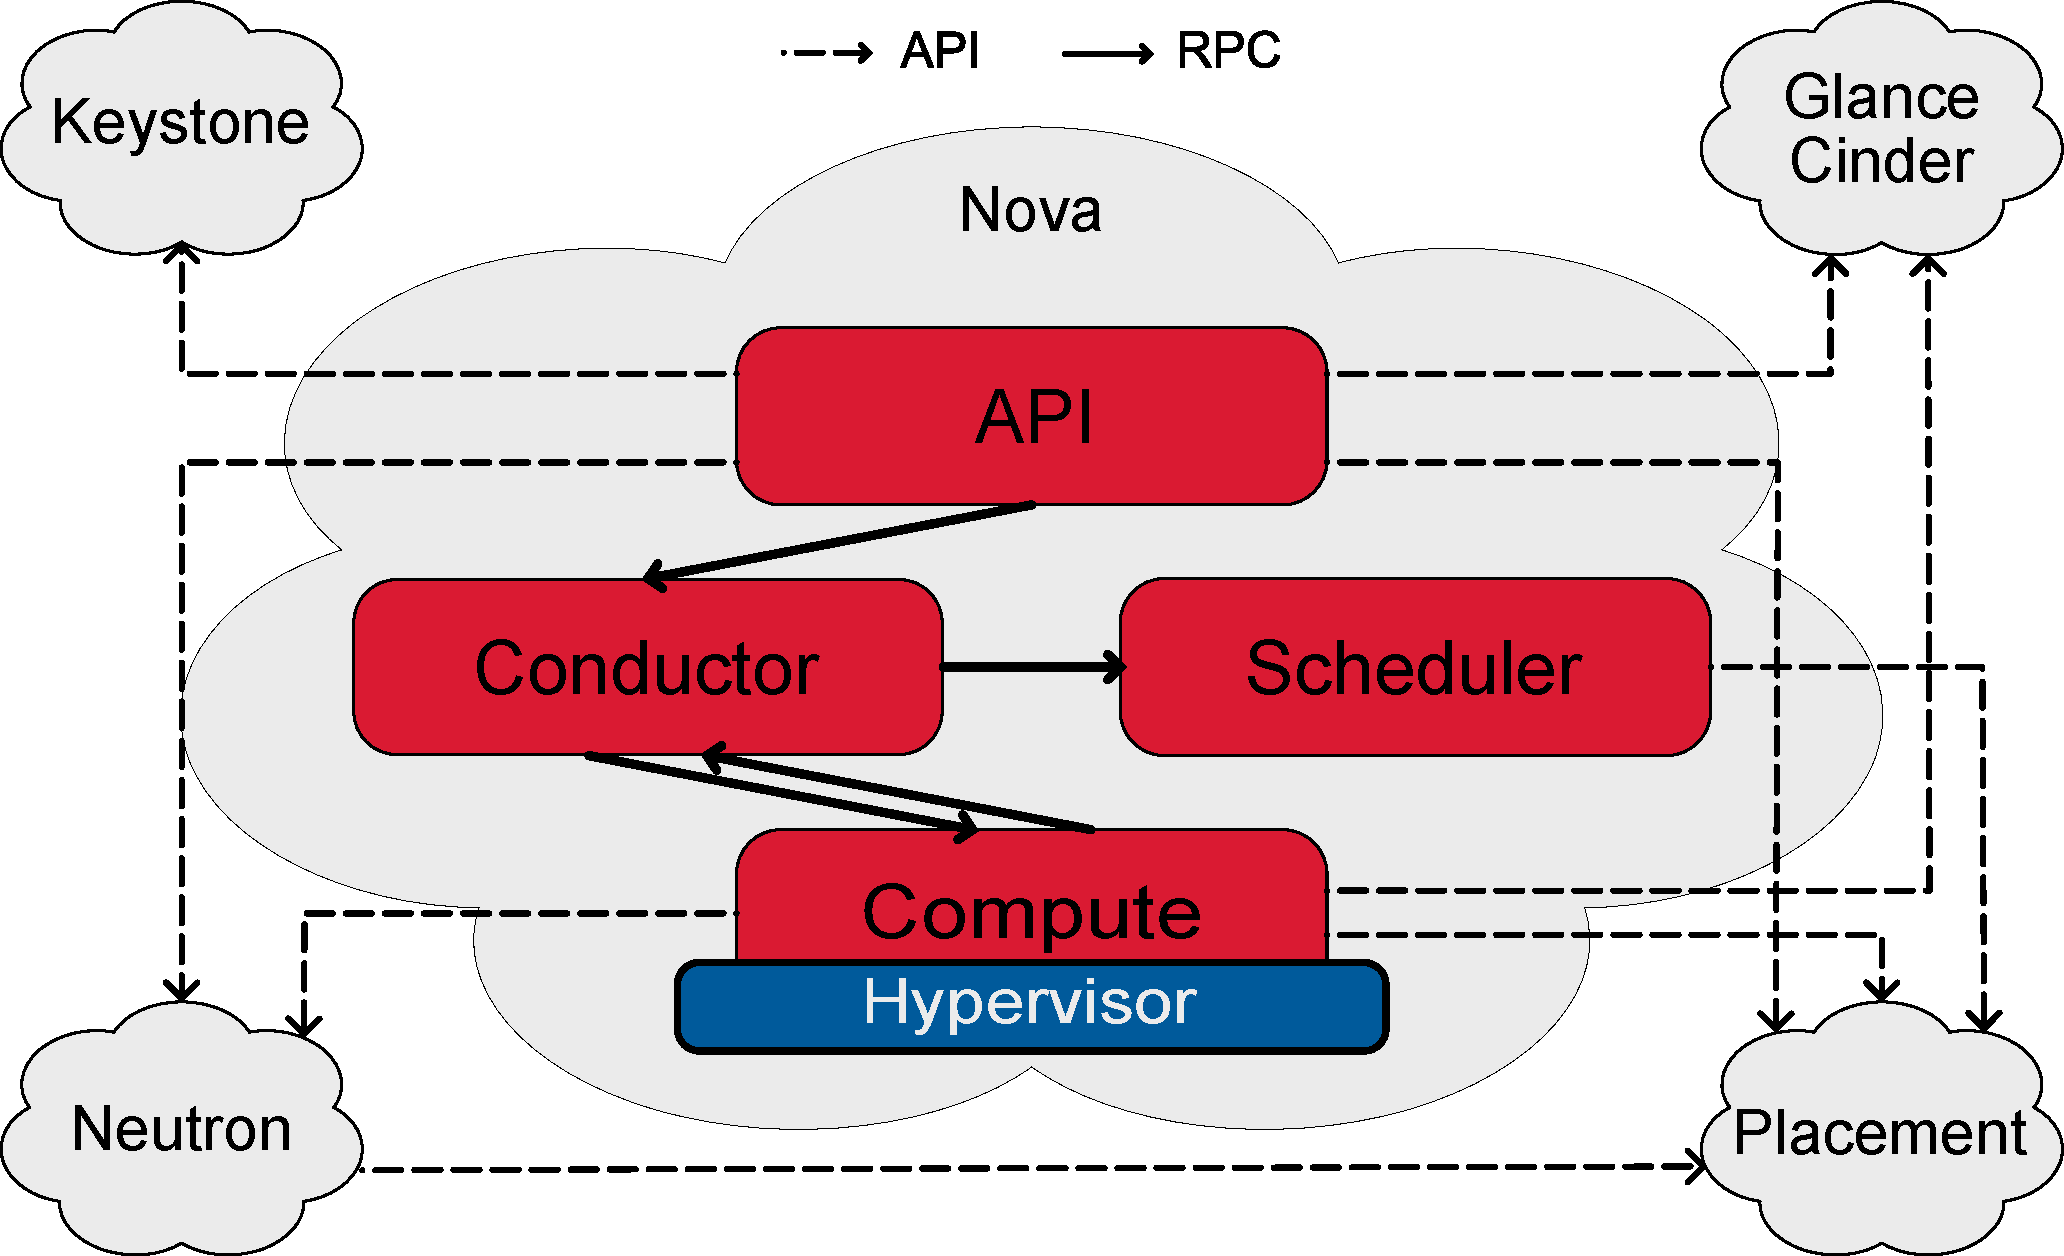
\includegraphics[width=0.7\textwidth ]{02_nova-architecture.pdf} 
                        \caption[OpenStack Nova architecture]{OpenStack Nova architecture \cite{OpenStackNSA2019}}
                        \label{figure:nova_architecture}
                    \end{center}	
                 \end{figure}
                 
                 
             \subsubsection{Networking Services}
             
                For the networking services, the OpenStack component \textsl{Neutron} is responsible.
                It focuses upon the delivery of Networking-as-a-Service to other OpenStack services, for example, to Nova-Compute instances.
                Neutron also supports creating multiple, on-demand networks along with all necessities like routers, switches, dynamic host configuration protocol, or domain name system services.
                 
                 
             \subsubsection{Storage Services}
                 
                OpenStack offers three different storage services.
                In this thesis, only the block-storage service \textsl{Cinder} will be considered.
                Cinder virtualizes and provides block-storage volumes to other components like Glance as well as for VMs themselves as storage.
                 

            
        \subsection{Communication Services}
            
            OpenStack communication mainly relies on two paradigms, which are used by all components and services.
            Following, \acp{API} and \acp{RPC} will be briefly described.
            
            \subsubsection{\acp{API}}
                
                All major OpenStack components contain an \ac{API} service.
                These \acp{API} expose one or more endpoints to the outside world to interact with.
                Other components and users themselves can use those endpoints to trigger actions or transfer data.
                The OpenStack command-line-tool and the Python \ac{SDK} make heavy use of the \ac{API} services to enable users to interact with OpenStack.
                
            
            \subsubsection{\acp{RPC}}
                
                Apart from \acp{API}, OpenStack heavily relies on \acp{RPC} for client-server intra-service communication. 
                For example, if the creation of a new \ac{VM} is requested, the Nova-Conductor (running on the controller) invokes Nova-Computer to build the \ac{VM} on a compute host via an \ac{RPC}.
                This is also indicated in Figure \ref{figure:nova_architecture}, where the communication inside the Nova component happens via \acp{RPC}, while the external communication happens via \acp{API}.
                The implementation of \acp{RPC} is achieved through the Advanced Message Queuing Protocol AMQP.
                All \acp{RPC} are packed into messages, which are then sent to a message broker, who further distributes the messages to the proper destinations.
                